\documentclass[1p]{elsarticle_modified}
%\bibliographystyle{elsarticle-num}

%\usepackage[colorlinks]{hyperref}
%\usepackage{abbrmath_seonhwa} %\Abb, \Ascr, \Acal ,\Abf, \Afrak
\usepackage{amsfonts}
\usepackage{amssymb}
\usepackage{amsmath}
\usepackage{amsthm}
\usepackage{scalefnt}
\usepackage{amsbsy}
\usepackage{kotex}
\usepackage{caption}
\usepackage{subfig}
\usepackage{color}
\usepackage{graphicx}
\usepackage{xcolor} %% white, black, red, green, blue, cyan, magenta, yellow
\usepackage{float}
\usepackage{setspace}
\usepackage{hyperref}

\usepackage{tikz}
\usetikzlibrary{arrows}

\usepackage{multirow}
\usepackage{array} % fixed length table
\usepackage{hhline}

%%%%%%%%%%%%%%%%%%%%%
\makeatletter
\renewcommand*\env@matrix[1][\arraystretch]{%
	\edef\arraystretch{#1}%
	\hskip -\arraycolsep
	\let\@ifnextchar\new@ifnextchar
	\array{*\c@MaxMatrixCols c}}
\makeatother %https://tex.stackexchange.com/questions/14071/how-can-i-increase-the-line-spacing-in-a-matrix
%%%%%%%%%%%%%%%

\usepackage[normalem]{ulem}

\newcommand{\msout}[1]{\ifmmode\text{\sout{\ensuremath{#1}}}\else\sout{#1}\fi}
%SOURCE: \msout is \stkout macro in https://tex.stackexchange.com/questions/20609/strikeout-in-math-mode

\newcommand{\cancel}[1]{
	\ifmmode
	{\color{red}\msout{#1}}
	\else
	{\color{red}\sout{#1}}
	\fi
}

\newcommand{\add}[1]{
	{\color{blue}\uwave{#1}}
}

\newcommand{\replace}[2]{
	\ifmmode
	{\color{red}\msout{#1}}{\color{blue}\uwave{#2}}
	\else
	{\color{red}\sout{#1}}{\color{blue}\uwave{#2}}
	\fi
}

\newcommand{\Sol}{\mathcal{S}} %segment
\newcommand{\D}{D} %diagram
\newcommand{\A}{\mathcal{A}} %arc


%%%%%%%%%%%%%%%%%%%%%%%%%%%%%5 test

\def\sl{\operatorname{\textup{SL}}(2,\Cbb)}
\def\psl{\operatorname{\textup{PSL}}(2,\Cbb)}
\def\quan{\mkern 1mu \triangleright \mkern 1mu}

\theoremstyle{definition}
\newtheorem{thm}{Theorem}[section]
\newtheorem{prop}[thm]{Proposition}
\newtheorem{lem}[thm]{Lemma}
\newtheorem{ques}[thm]{Question}
\newtheorem{cor}[thm]{Corollary}
\newtheorem{defn}[thm]{Definition}
\newtheorem{exam}[thm]{Example}
\newtheorem{rmk}[thm]{Remark}
\newtheorem{alg}[thm]{Algorithm}

\newcommand{\I}{\sqrt{-1}}
\begin{document}

%\begin{frontmatter}
%
%\title{Boundary parabolic representations of knots up to 8 crossings}
%
%%% Group authors per affiliation:
%\author{Yunhi Cho} 
%\address{Department of Mathematics, University of Seoul, Seoul, Korea}
%\ead{yhcho@uos.ac.kr}
%
%
%\author{Seonhwa Kim} %\fnref{s_kim}}
%\address{Center for Geometry and Physics, Institute for Basic Science, Pohang, 37673, Korea}
%\ead{ryeona17@ibs.re.kr}
%
%\author{Hyuk Kim}
%\address{Department of Mathematical Sciences, Seoul National University, Seoul 08826, Korea}
%\ead{hyukkim@snu.ac.kr}
%
%\author{Seokbeom Yoon}
%\address{Department of Mathematical Sciences, Seoul National University, Seoul, 08826,  Korea}
%\ead{sbyoon15@snu.ac.kr}
%
%\begin{abstract}
%We find all boundary parabolic representation of knots up to 8 crossings.
%
%\end{abstract}
%\begin{keyword}
%    \MSC[2010] 57M25 
%\end{keyword}
%
%\end{frontmatter}

%\linenumbers
%\tableofcontents
%
\newcommand\colored[1]{\textcolor{white}{\rule[-0.35ex]{0.8em}{1.4ex}}\kern-0.8em\color{red} #1}%
%\newcommand\colored[1]{\textcolor{white}{ #1}\kern-2.17ex	\textcolor{white}{ #1}\kern-1.81ex	\textcolor{white}{ #1}\kern-2.15ex\color{red}#1	}

{\Large $\underline{12a_{0144}~(K12a_{0144})}$}

\setlength{\tabcolsep}{10pt}
\renewcommand{\arraystretch}{1.6}
\vspace{1cm}\begin{tabular}{m{100pt}>{\centering\arraybackslash}m{274pt}}
\multirow{5}{120pt}{
	\centering
	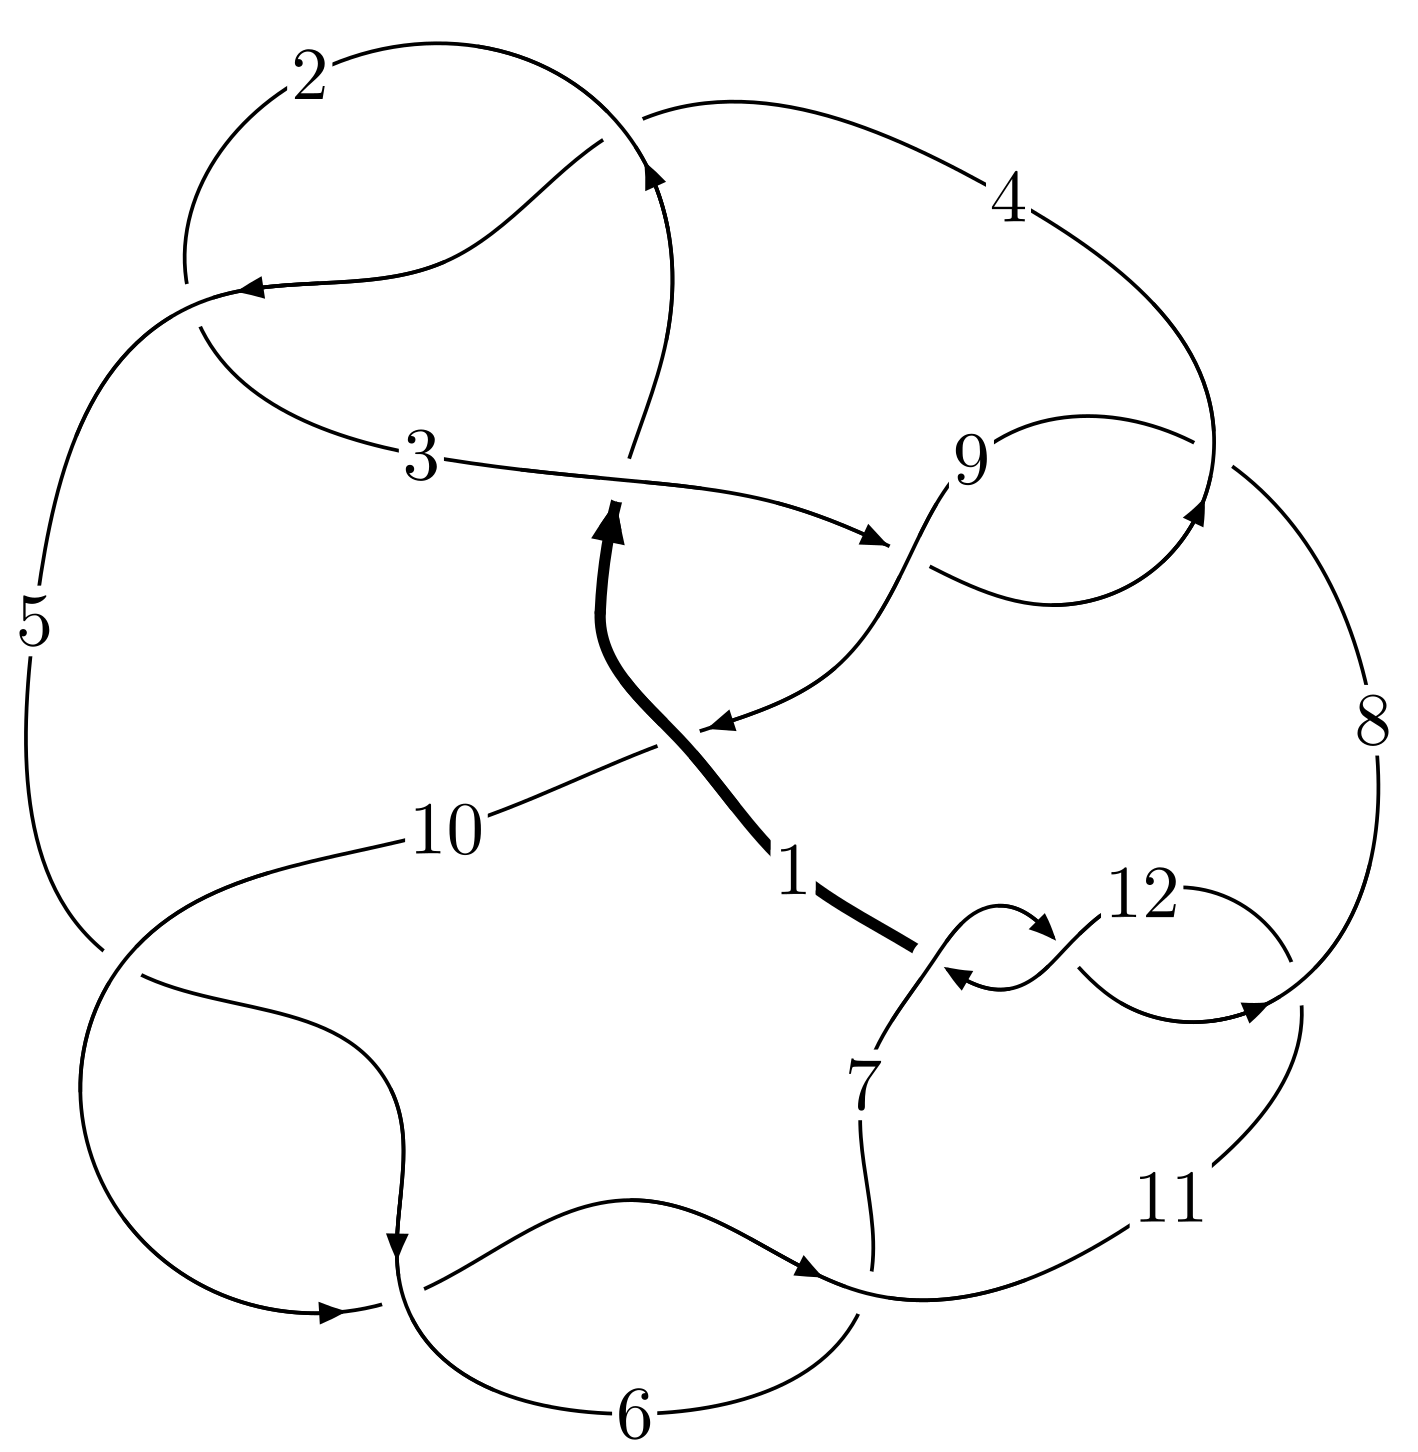
\includegraphics[width=112pt]{../../../GIT/diagram.site/Diagrams/png/945_12a_0144.png}\\
\ \ \ A knot diagram\footnotemark}&
\allowdisplaybreaks
\textbf{Linearized knot diagam} \\
\cline{2-2}
 &
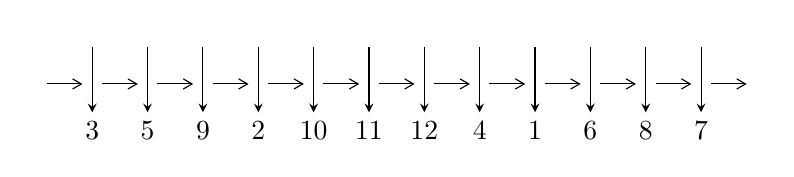
\begin{tikzpicture}[x=20pt, y=17pt]
	% nodes
	\node (C0) at (0, 0) {};
	\node (C1) at (1, 0) {};
	\node (C1U) at (1, +1) {};
	\node (C1D) at (1, -1) {3};

	\node (C2) at (2, 0) {};
	\node (C2U) at (2, +1) {};
	\node (C2D) at (2, -1) {5};

	\node (C3) at (3, 0) {};
	\node (C3U) at (3, +1) {};
	\node (C3D) at (3, -1) {9};

	\node (C4) at (4, 0) {};
	\node (C4U) at (4, +1) {};
	\node (C4D) at (4, -1) {2};

	\node (C5) at (5, 0) {};
	\node (C5U) at (5, +1) {};
	\node (C5D) at (5, -1) {10};

	\node (C6) at (6, 0) {};
	\node (C6U) at (6, +1) {};
	\node (C6D) at (6, -1) {11};

	\node (C7) at (7, 0) {};
	\node (C7U) at (7, +1) {};
	\node (C7D) at (7, -1) {12};

	\node (C8) at (8, 0) {};
	\node (C8U) at (8, +1) {};
	\node (C8D) at (8, -1) {4};

	\node (C9) at (9, 0) {};
	\node (C9U) at (9, +1) {};
	\node (C9D) at (9, -1) {1};

	\node (C10) at (10, 0) {};
	\node (C10U) at (10, +1) {};
	\node (C10D) at (10, -1) {6};

	\node (C11) at (11, 0) {};
	\node (C11U) at (11, +1) {};
	\node (C11D) at (11, -1) {8};

	\node (C12) at (12, 0) {};
	\node (C12U) at (12, +1) {};
	\node (C12D) at (12, -1) {7};
	\node (C13) at (13, 0) {};

	% arrows
	\draw[->,>={angle 60}]
	(C0) edge (C1) (C1) edge (C2) (C2) edge (C3) (C3) edge (C4) (C4) edge (C5) (C5) edge (C6) (C6) edge (C7) (C7) edge (C8) (C8) edge (C9) (C9) edge (C10) (C10) edge (C11) (C11) edge (C12) (C12) edge (C13) ;	\draw[->,>=stealth]
	(C1U) edge (C1D) (C2U) edge (C2D) (C3U) edge (C3D) (C4U) edge (C4D) (C5U) edge (C5D) (C6U) edge (C6D) (C7U) edge (C7D) (C8U) edge (C8D) (C9U) edge (C9D) (C10U) edge (C10D) (C11U) edge (C11D) (C12U) edge (C12D) ;
	\end{tikzpicture} \\
\hhline{~~} \\& 
\textbf{Solving Sequence} \\ \cline{2-2} 
 &
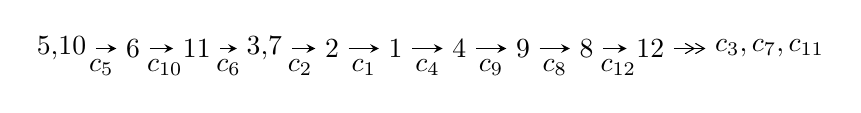
\begin{tikzpicture}[x=23pt, y=7pt]
	% node
	\node (A0) at (-1/8, 0) {5,10};
	\node (A1) at (1, 0) {6};
	\node (A2) at (2, 0) {11};
	\node (A3) at (49/16, 0) {3,7};
	\node (A4) at (33/8, 0) {2};
	\node (A5) at (41/8, 0) {1};
	\node (A6) at (49/8, 0) {4};
	\node (A7) at (57/8, 0) {9};
	\node (A8) at (65/8, 0) {8};
	\node (A9) at (73/8, 0) {12};
	\node (C1) at (1/2, -1) {$c_{5}$};
	\node (C2) at (3/2, -1) {$c_{10}$};
	\node (C3) at (5/2, -1) {$c_{6}$};
	\node (C4) at (29/8, -1) {$c_{2}$};
	\node (C5) at (37/8, -1) {$c_{1}$};
	\node (C6) at (45/8, -1) {$c_{4}$};
	\node (C7) at (53/8, -1) {$c_{9}$};
	\node (C8) at (61/8, -1) {$c_{8}$};
	\node (C9) at (69/8, -1) {$c_{12}$};
	\node (A10) at (11, 0) {$c_{3},c_{7},c_{11}$};

	% edge
	\draw[->,>=stealth]	
	(A0) edge (A1) (A1) edge (A2) (A2) edge (A3) (A3) edge (A4) (A4) edge (A5) (A5) edge (A6) (A6) edge (A7) (A7) edge (A8) (A8) edge (A9) ;
	\draw[->>,>={angle 60}]	
	(A9) edge (A10);
\end{tikzpicture} \\ 

\end{tabular} \\

\footnotetext{
The image of knot diagram is generated by the software ``\textbf{Draw programme}" developed by Andrew Bartholomew(\url{http://www.layer8.co.uk/maths/draw/index.htm\#Running-draw}), where we modified some parts for our purpose(\url{https://github.com/CATsTAILs/LinksPainter}).
}\phantom \\ \newline 
\centering \textbf{Ideals for irreducible components\footnotemark of $X_{\text{par}}$} 
 
\begin{align*}
I^u_{1}&=\langle 
-1.00279\times10^{169} u^{80}+6.54285\times10^{169} u^{79}+\cdots+5.58362\times10^{170} b-5.37338\times10^{170},\\
\phantom{I^u_{1}}&\phantom{= \langle  }2.70498\times10^{170} u^{80}+4.42960\times10^{170} u^{79}+\cdots+1.67509\times10^{171} a+1.36068\times10^{171},\;u^{81}+2 u^{80}+\cdots-27 u-9\rangle \\
I^u_{2}&=\langle 
b+1,\;a+1,\;u^6- u^5-3 u^4+2 u^3+2 u^2+u-1\rangle \\
\\
\end{align*}
\raggedright * 2 irreducible components of $\dim_{\mathbb{C}}=0$, with total 87 representations.\\
\footnotetext{All coefficients of polynomials are rational numbers. But the coefficients are sometimes approximated in decimal forms when there is not enough margin.}
\newpage
\renewcommand{\arraystretch}{1}
\centering \section*{I. $I^u_{1}= \langle -1.00\times10^{169} u^{80}+6.54\times10^{169} u^{79}+\cdots+5.58\times10^{170} b-5.37\times10^{170},\;2.70\times10^{170} u^{80}+4.43\times10^{170} u^{79}+\cdots+1.68\times10^{171} a+1.36\times10^{171},\;u^{81}+2 u^{80}+\cdots-27 u-9 \rangle$}
\flushleft \textbf{(i) Arc colorings}\\
\begin{tabular}{m{7pt} m{180pt} m{7pt} m{180pt} }
\flushright $a_{5}=$&$\begin{pmatrix}1\\0\end{pmatrix}$ \\
\flushright $a_{10}=$&$\begin{pmatrix}0\\u\end{pmatrix}$ \\
\flushright $a_{6}=$&$\begin{pmatrix}1\\u^2\end{pmatrix}$ \\
\flushright $a_{11}=$&$\begin{pmatrix}- u\\- u^3+u\end{pmatrix}$ \\
\flushright $a_{3}=$&$\begin{pmatrix}-0.161483 u^{80}-0.264440 u^{79}+\cdots-4.05452 u-0.812307\\0.0179595 u^{80}-0.117179 u^{79}+\cdots-1.66032 u+0.962347\end{pmatrix}$ \\
\flushright $a_{7}=$&$\begin{pmatrix}- u^2+1\\- u^4+2 u^2\end{pmatrix}$ \\
\flushright $a_{2}=$&$\begin{pmatrix}-0.143524 u^{80}-0.381620 u^{79}+\cdots-5.71484 u+0.150039\\0.0179595 u^{80}-0.117179 u^{79}+\cdots-1.66032 u+0.962347\end{pmatrix}$ \\
\flushright $a_{1}=$&$\begin{pmatrix}-0.428496 u^{80}-0.583915 u^{79}+\cdots+12.7602 u+6.52385\\-0.131228 u^{80}-0.0542263 u^{79}+\cdots+3.05402 u+0.800318\end{pmatrix}$ \\
\flushright $a_{4}=$&$\begin{pmatrix}0.259446 u^{80}+0.204971 u^{79}+\cdots-18.6233 u-5.57768\\0.157772 u^{80}+0.183340 u^{79}+\cdots-4.83114 u-3.19296\end{pmatrix}$ \\
\flushright $a_{9}=$&$\begin{pmatrix}0.111704 u^{80}+0.397558 u^{79}+\cdots-6.23678 u-4.64153\\0.0545258 u^{80}+0.0419649 u^{79}+\cdots-0.269902 u-0.998356\end{pmatrix}$ \\
\flushright $a_{8}=$&$\begin{pmatrix}0.184153 u^{80}+0.220811 u^{79}+\cdots-11.7267 u-4.50953\\0.273077 u^{80}+0.267431 u^{79}+\cdots-5.04554 u-3.85646\end{pmatrix}$ \\
\flushright $a_{12}=$&$\begin{pmatrix}-0.493301 u^{80}-0.569619 u^{79}+\cdots+16.6789 u+6.41142\\0.0147144 u^{80}+0.0729091 u^{79}+\cdots+0.464872 u-0.795811\end{pmatrix}$\\&\end{tabular}
\flushleft \textbf{(ii) Obstruction class $= -1$}\\~\\
\flushleft \textbf{(iii) Cusp Shapes $= -0.191745 u^{80}-0.688940 u^{79}+\cdots+3.61897 u-7.41512$}\\~\\
\newpage\renewcommand{\arraystretch}{1}
\flushleft \textbf{(iv) u-Polynomials at the component}\newline \\
\begin{tabular}{m{50pt}|m{274pt}}
Crossings & \hspace{64pt}u-Polynomials at each crossing \\
\hline $$\begin{aligned}c_{1}\end{aligned}$$&$\begin{aligned}
&u^{81}+39 u^{80}+\cdots+52 u+1
\end{aligned}$\\
\hline $$\begin{aligned}c_{2},c_{4}\end{aligned}$$&$\begin{aligned}
&u^{81}-7 u^{80}+\cdots+2 u+1
\end{aligned}$\\
\hline $$\begin{aligned}c_{3},c_{8}\end{aligned}$$&$\begin{aligned}
&u^{81}- u^{80}+\cdots+64 u+64
\end{aligned}$\\
\hline $$\begin{aligned}c_{5},c_{6},c_{10}\end{aligned}$$&$\begin{aligned}
&u^{81}-2 u^{80}+\cdots-27 u+9
\end{aligned}$\\
\hline $$\begin{aligned}c_{7},c_{11},c_{12}\end{aligned}$$&$\begin{aligned}
&u^{81}+2 u^{80}+\cdots+3 u+1
\end{aligned}$\\
\hline $$\begin{aligned}c_{9}\end{aligned}$$&$\begin{aligned}
&u^{81}+8 u^{80}+\cdots-3141 u+2537
\end{aligned}$\\
\hline
\end{tabular}\\~\\
\newpage\renewcommand{\arraystretch}{1}
\flushleft \textbf{(v) Riley Polynomials at the component}\newline \\
\begin{tabular}{m{50pt}|m{274pt}}
Crossings & \hspace{64pt}Riley Polynomials at each crossing \\
\hline $$\begin{aligned}c_{1}\end{aligned}$$&$\begin{aligned}
&y^{81}+13 y^{80}+\cdots+3164 y-1
\end{aligned}$\\
\hline $$\begin{aligned}c_{2},c_{4}\end{aligned}$$&$\begin{aligned}
&y^{81}-39 y^{80}+\cdots+52 y-1
\end{aligned}$\\
\hline $$\begin{aligned}c_{3},c_{8}\end{aligned}$$&$\begin{aligned}
&y^{81}+39 y^{80}+\cdots-40960 y-4096
\end{aligned}$\\
\hline $$\begin{aligned}c_{5},c_{6},c_{10}\end{aligned}$$&$\begin{aligned}
&y^{81}-80 y^{80}+\cdots-693 y-81
\end{aligned}$\\
\hline $$\begin{aligned}c_{7},c_{11},c_{12}\end{aligned}$$&$\begin{aligned}
&y^{81}+64 y^{80}+\cdots+11 y-1
\end{aligned}$\\
\hline $$\begin{aligned}c_{9}\end{aligned}$$&$\begin{aligned}
&y^{81}+4 y^{80}+\cdots+43125951 y-6436369
\end{aligned}$\\
\hline
\end{tabular}\\~\\
\newpage\flushleft \textbf{(vi) Complex Volumes and Cusp Shapes}
$$\begin{array}{c|c|c}  
\text{Solutions to }I^u_{1}& \I (\text{vol} + \sqrt{-1}CS) & \text{Cusp shape}\\
 \hline 
\begin{aligned}
u &= \phantom{-}0.549854 + 0.817265 I \\
a &= -0.668883 + 0.232142 I \\
b &= -1.240880 + 0.079920 I\end{aligned}
 & \phantom{-}2.18909 - 2.68944 I & \phantom{-0.000000 } 0 \\ \hline\begin{aligned}
u &= \phantom{-}0.549854 - 0.817265 I \\
a &= -0.668883 - 0.232142 I \\
b &= -1.240880 - 0.079920 I\end{aligned}
 & \phantom{-}2.18909 + 2.68944 I & \phantom{-0.000000 } 0 \\ \hline\begin{aligned}
u &= -0.423119 + 0.878378 I \\
a &= \phantom{-}0.92747 + 1.27632 I \\
b &= -0.735616 - 0.474491 I\end{aligned}
 & \phantom{-}3.90058 + 0.83925 I & \phantom{-0.000000 } 0 \\ \hline\begin{aligned}
u &= -0.423119 - 0.878378 I \\
a &= \phantom{-}0.92747 - 1.27632 I \\
b &= -0.735616 + 0.474491 I\end{aligned}
 & \phantom{-}3.90058 - 0.83925 I & \phantom{-0.000000 } 0 \\ \hline\begin{aligned}
u &= -0.629386 + 0.882957 I \\
a &= \phantom{-}0.11503 - 1.99991 I \\
b &= -0.920437 + 0.512641 I\end{aligned}
 & \phantom{-}3.30143 + 4.94717 I & \phantom{-0.000000 } 0 \\ \hline\begin{aligned}
u &= -0.629386 - 0.882957 I \\
a &= \phantom{-}0.11503 + 1.99991 I \\
b &= -0.920437 - 0.512641 I\end{aligned}
 & \phantom{-}3.30143 - 4.94717 I & \phantom{-0.000000 } 0 \\ \hline\begin{aligned}
u &= \phantom{-}0.871043 + 0.244839 I \\
a &= \phantom{-}0.226267 - 0.008099 I \\
b &= \phantom{-}0.923001 - 0.532162 I\end{aligned}
 & -1.18559 + 2.18588 I & \phantom{-0.000000 } 0 \\ \hline\begin{aligned}
u &= \phantom{-}0.871043 - 0.244839 I \\
a &= \phantom{-}0.226267 + 0.008099 I \\
b &= \phantom{-}0.923001 + 0.532162 I\end{aligned}
 & -1.18559 - 2.18588 I & \phantom{-0.000000 } 0 \\ \hline\begin{aligned}
u &= \phantom{-}0.285149 + 1.085700 I \\
a &= -0.262963 + 1.112650 I \\
b &= \phantom{-}1.035310 - 0.663440 I\end{aligned}
 & \phantom{-}7.49110 + 4.12587 I & \phantom{-0.000000 } 0 \\ \hline\begin{aligned}
u &= \phantom{-}0.285149 - 1.085700 I \\
a &= -0.262963 - 1.112650 I \\
b &= \phantom{-}1.035310 + 0.663440 I\end{aligned}
 & \phantom{-}7.49110 - 4.12587 I & \phantom{-0.000000 } 0\\
 \hline 
 \end{array}$$\newpage$$\begin{array}{c|c|c}  
\text{Solutions to }I^u_{1}& \I (\text{vol} + \sqrt{-1}CS) & \text{Cusp shape}\\
 \hline 
\begin{aligned}
u &= \phantom{-}0.404547 + 1.051810 I \\
a &= -0.220162 - 1.151750 I \\
b &= \phantom{-}0.573320 + 0.814273 I\end{aligned}
 & \phantom{-}8.88154 - 1.39549 I & \phantom{-0.000000 } 0 \\ \hline\begin{aligned}
u &= \phantom{-}0.404547 - 1.051810 I \\
a &= -0.220162 + 1.151750 I \\
b &= \phantom{-}0.573320 - 0.814273 I\end{aligned}
 & \phantom{-}8.88154 + 1.39549 I & \phantom{-0.000000 } 0 \\ \hline\begin{aligned}
u &= \phantom{-}0.669709 + 0.987448 I \\
a &= -0.659904 + 0.714844 I \\
b &= \phantom{-}0.453835 - 0.861154 I\end{aligned}
 & \phantom{-}8.12466 - 5.17001 I & \phantom{-0.000000 } 0 \\ \hline\begin{aligned}
u &= \phantom{-}0.669709 - 0.987448 I \\
a &= -0.659904 - 0.714844 I \\
b &= \phantom{-}0.453835 + 0.861154 I\end{aligned}
 & \phantom{-}8.12466 + 5.17001 I & \phantom{-0.000000 } 0 \\ \hline\begin{aligned}
u &= -0.743128 + 0.238456 I \\
a &= \phantom{-}0.936570 - 0.552245 I \\
b &= \phantom{-}0.670993 + 0.510713 I\end{aligned}
 & \phantom{-}2.69972 + 1.11767 I & -8.46846 - 0.34647 I \\ \hline\begin{aligned}
u &= -0.743128 - 0.238456 I \\
a &= \phantom{-}0.936570 + 0.552245 I \\
b &= \phantom{-}0.670993 - 0.510713 I\end{aligned}
 & \phantom{-}2.69972 - 1.11767 I & -8.46846 + 0.34647 I \\ \hline\begin{aligned}
u &= -0.528811 + 0.566420 I \\
a &= \phantom{-}0.30265 + 2.22515 I \\
b &= \phantom{-}1.101470 - 0.618329 I\end{aligned}
 & \phantom{-}0.93164 + 8.30570 I & -13.1243 - 9.3739 I \\ \hline\begin{aligned}
u &= -0.528811 - 0.566420 I \\
a &= \phantom{-}0.30265 - 2.22515 I \\
b &= \phantom{-}1.101470 + 0.618329 I\end{aligned}
 & \phantom{-}0.93164 - 8.30570 I & -13.1243 + 9.3739 I \\ \hline\begin{aligned}
u &= \phantom{-}0.761650 + 0.974344 I \\
a &= \phantom{-}0.37235 - 1.64135 I \\
b &= \phantom{-}1.113920 + 0.647715 I\end{aligned}
 & \phantom{-}6.14001 - 10.75700 I & \phantom{-0.000000 } 0 \\ \hline\begin{aligned}
u &= \phantom{-}0.761650 - 0.974344 I \\
a &= \phantom{-}0.37235 + 1.64135 I \\
b &= \phantom{-}1.113920 - 0.647715 I\end{aligned}
 & \phantom{-}6.14001 + 10.75700 I & \phantom{-0.000000 } 0\\
 \hline 
 \end{array}$$\newpage$$\begin{array}{c|c|c}  
\text{Solutions to }I^u_{1}& \I (\text{vol} + \sqrt{-1}CS) & \text{Cusp shape}\\
 \hline 
\begin{aligned}
u &= \phantom{-}1.245470 + 0.133358 I \\
a &= \phantom{-}0.291110 - 0.847829 I \\
b &= \phantom{-}0.746809 + 0.711067 I\end{aligned}
 & -0.83961 - 2.58594 I & \phantom{-0.000000 } 0 \\ \hline\begin{aligned}
u &= \phantom{-}1.245470 - 0.133358 I \\
a &= \phantom{-}0.291110 + 0.847829 I \\
b &= \phantom{-}0.746809 - 0.711067 I\end{aligned}
 & -0.83961 + 2.58594 I & \phantom{-0.000000 } 0 \\ \hline\begin{aligned}
u &= -1.202630 + 0.422167 I \\
a &= \phantom{-}0.159393 - 0.613266 I \\
b &= \phantom{-}0.866243 + 0.666328 I\end{aligned}
 & \phantom{-}2.92901 + 1.26794 I & \phantom{-0.000000 } 0 \\ \hline\begin{aligned}
u &= -1.202630 - 0.422167 I \\
a &= \phantom{-}0.159393 + 0.613266 I \\
b &= \phantom{-}0.866243 - 0.666328 I\end{aligned}
 & \phantom{-}2.92901 - 1.26794 I & \phantom{-0.000000 } 0 \\ \hline\begin{aligned}
u &= -0.434384 + 0.537078 I \\
a &= -1.142120 - 0.805181 I \\
b &= \phantom{-}0.438054 + 0.799462 I\end{aligned}
 & \phantom{-}2.90437 + 2.98477 I & -9.55591 - 5.23848 I \\ \hline\begin{aligned}
u &= -0.434384 - 0.537078 I \\
a &= -1.142120 + 0.805181 I \\
b &= \phantom{-}0.438054 - 0.799462 I\end{aligned}
 & \phantom{-}2.90437 - 2.98477 I & -9.55591 + 5.23848 I \\ \hline\begin{aligned}
u &= -1.312810 + 0.029010 I \\
a &= -0.553493 - 0.125261 I \\
b &= \phantom{-}0.324181 + 0.863693 I\end{aligned}
 & \phantom{-}0.185868 + 1.219880 I & \phantom{-0.000000 } 0 \\ \hline\begin{aligned}
u &= -1.312810 - 0.029010 I \\
a &= -0.553493 + 0.125261 I \\
b &= \phantom{-}0.324181 - 0.863693 I\end{aligned}
 & \phantom{-}0.185868 - 1.219880 I & \phantom{-0.000000 } 0 \\ \hline\begin{aligned}
u &= \phantom{-}1.359630 + 0.023425 I \\
a &= -0.90230 - 1.79054 I \\
b &= -1.053060 + 0.510916 I\end{aligned}
 & -4.34022 + 0.45005 I & \phantom{-0.000000 } 0 \\ \hline\begin{aligned}
u &= \phantom{-}1.359630 - 0.023425 I \\
a &= -0.90230 + 1.79054 I \\
b &= -1.053060 - 0.510916 I\end{aligned}
 & -4.34022 - 0.45005 I & \phantom{-0.000000 } 0\\
 \hline 
 \end{array}$$\newpage$$\begin{array}{c|c|c}  
\text{Solutions to }I^u_{1}& \I (\text{vol} + \sqrt{-1}CS) & \text{Cusp shape}\\
 \hline 
\begin{aligned}
u &= -1.364690 + 0.077002 I \\
a &= \phantom{-}1.17174 + 1.47880 I \\
b &= \phantom{-}1.160950 - 0.604080 I\end{aligned}
 & -2.30932 + 6.62917 I & \phantom{-0.000000 } 0 \\ \hline\begin{aligned}
u &= -1.364690 - 0.077002 I \\
a &= \phantom{-}1.17174 - 1.47880 I \\
b &= \phantom{-}1.160950 + 0.604080 I\end{aligned}
 & -2.30932 - 6.62917 I & \phantom{-0.000000 } 0 \\ \hline\begin{aligned}
u &= \phantom{-}0.457361 + 0.415520 I \\
a &= \phantom{-}0.10898 + 2.86219 I \\
b &= -0.946808 - 0.440327 I\end{aligned}
 & -1.58018 - 2.82736 I & -15.3914 + 7.4030 I \\ \hline\begin{aligned}
u &= \phantom{-}0.457361 - 0.415520 I \\
a &= \phantom{-}0.10898 - 2.86219 I \\
b &= -0.946808 + 0.440327 I\end{aligned}
 & -1.58018 + 2.82736 I & -15.3914 - 7.4030 I \\ \hline\begin{aligned}
u &= -1.383020 + 0.067923 I \\
a &= -1.162760 + 0.218155 I \\
b &= -1.266990 + 0.222352 I\end{aligned}
 & -5.03426 + 2.16541 I & \phantom{-0.000000 } 0 \\ \hline\begin{aligned}
u &= -1.383020 - 0.067923 I \\
a &= -1.162760 - 0.218155 I \\
b &= -1.266990 - 0.222352 I\end{aligned}
 & -5.03426 - 2.16541 I & \phantom{-0.000000 } 0 \\ \hline\begin{aligned}
u &= \phantom{-}1.378230 + 0.145858 I \\
a &= \phantom{-}0.679555 + 0.442834 I \\
b &= -0.377108 - 0.555718 I\end{aligned}
 & -2.43296 - 3.85164 I & \phantom{-0.000000 } 0 \\ \hline\begin{aligned}
u &= \phantom{-}1.378230 - 0.145858 I \\
a &= \phantom{-}0.679555 - 0.442834 I \\
b &= -0.377108 + 0.555718 I\end{aligned}
 & -2.43296 + 3.85164 I & \phantom{-0.000000 } 0 \\ \hline\begin{aligned}
u &= -0.327143 + 0.472697 I \\
a &= \phantom{-}0.912647 + 0.072753 I \\
b &= \phantom{-}0.063180 + 0.313296 I\end{aligned}
 & \phantom{-}2.85428 + 1.54452 I & -7.25846 - 4.25517 I \\ \hline\begin{aligned}
u &= -0.327143 - 0.472697 I \\
a &= \phantom{-}0.912647 - 0.072753 I \\
b &= \phantom{-}0.063180 - 0.313296 I\end{aligned}
 & \phantom{-}2.85428 - 1.54452 I & -7.25846 + 4.25517 I\\
 \hline 
 \end{array}$$\newpage$$\begin{array}{c|c|c}  
\text{Solutions to }I^u_{1}& \I (\text{vol} + \sqrt{-1}CS) & \text{Cusp shape}\\
 \hline 
\begin{aligned}
u &= -1.44455 + 0.07637 I \\
a &= \phantom{-}0.681802 + 0.524693 I \\
b &= -0.430423 - 0.562966 I\end{aligned}
 & -6.23300 + 0.57167 I & \phantom{-0.000000 } 0 \\ \hline\begin{aligned}
u &= -1.44455 - 0.07637 I \\
a &= \phantom{-}0.681802 - 0.524693 I \\
b &= -0.430423 + 0.562966 I\end{aligned}
 & -6.23300 - 0.57167 I & \phantom{-0.000000 } 0 \\ \hline\begin{aligned}
u &= -1.38481 + 0.42788 I \\
a &= \phantom{-}0.190392 + 0.906474 I \\
b &= \phantom{-}0.729122 - 0.763915 I\end{aligned}
 & \phantom{-}3.37635 + 6.67232 I & \phantom{-0.000000 } 0 \\ \hline\begin{aligned}
u &= -1.38481 - 0.42788 I \\
a &= \phantom{-}0.190392 - 0.906474 I \\
b &= \phantom{-}0.729122 + 0.763915 I\end{aligned}
 & \phantom{-}3.37635 - 6.67232 I & \phantom{-0.000000 } 0 \\ \hline\begin{aligned}
u &= -0.166020 + 0.514578 I \\
a &= -0.44693 + 1.85551 I \\
b &= \phantom{-}0.518731 - 0.743814 I\end{aligned}
 & \phantom{-}3.42589 + 0.03376 I & -7.43382 - 3.19727 I \\ \hline\begin{aligned}
u &= -0.166020 - 0.514578 I \\
a &= -0.44693 - 1.85551 I \\
b &= \phantom{-}0.518731 + 0.743814 I\end{aligned}
 & \phantom{-}3.42589 - 0.03376 I & -7.43382 + 3.19727 I \\ \hline\begin{aligned}
u &= -0.442772 + 0.285049 I \\
a &= -0.529533 - 0.735122 I \\
b &= -1.155150 - 0.126670 I\end{aligned}
 & -2.38286 + 0.75626 I & -14.3003 - 8.7966 I \\ \hline\begin{aligned}
u &= -0.442772 - 0.285049 I \\
a &= -0.529533 + 0.735122 I \\
b &= -1.155150 + 0.126670 I\end{aligned}
 & -2.38286 - 0.75626 I & -14.3003 + 8.7966 I \\ \hline\begin{aligned}
u &= -0.050728 + 0.520709 I \\
a &= -1.27689 - 1.67775 I \\
b &= \phantom{-}1.053540 + 0.606874 I\end{aligned}
 & \phantom{-}1.82638 - 5.10869 I & -10.33632 + 2.79274 I \\ \hline\begin{aligned}
u &= -0.050728 - 0.520709 I \\
a &= -1.27689 + 1.67775 I \\
b &= \phantom{-}1.053540 - 0.606874 I\end{aligned}
 & \phantom{-}1.82638 + 5.10869 I & -10.33632 - 2.79274 I\\
 \hline 
 \end{array}$$\newpage$$\begin{array}{c|c|c}  
\text{Solutions to }I^u_{1}& \I (\text{vol} + \sqrt{-1}CS) & \text{Cusp shape}\\
 \hline 
\begin{aligned}
u &= \phantom{-}1.48422 + 0.11960 I \\
a &= -1.091750 + 0.198604 I \\
b &= -1.280200 + 0.207550 I\end{aligned}
 & -8.74917 - 2.34681 I & \phantom{-0.000000 } 0 \\ \hline\begin{aligned}
u &= \phantom{-}1.48422 - 0.11960 I \\
a &= -1.091750 - 0.198604 I \\
b &= -1.280200 - 0.207550 I\end{aligned}
 & -8.74917 + 2.34681 I & \phantom{-0.000000 } 0 \\ \hline\begin{aligned}
u &= \phantom{-}1.48081 + 0.20261 I \\
a &= -0.517683 + 0.219188 I \\
b &= \phantom{-}0.336394 - 0.886288 I\end{aligned}
 & -3.35067 - 5.75212 I & \phantom{-0.000000 } 0 \\ \hline\begin{aligned}
u &= \phantom{-}1.48081 - 0.20261 I \\
a &= -0.517683 - 0.219188 I \\
b &= \phantom{-}0.336394 + 0.886288 I\end{aligned}
 & -3.35067 + 5.75212 I & \phantom{-0.000000 } 0 \\ \hline\begin{aligned}
u &= -1.48858 + 0.15570 I \\
a &= -0.76126 - 1.73875 I \\
b &= -1.043700 + 0.528714 I\end{aligned}
 & -7.98070 + 4.98123 I & \phantom{-0.000000 } 0 \\ \hline\begin{aligned}
u &= -1.48858 - 0.15570 I \\
a &= -0.76126 + 1.73875 I \\
b &= -1.043700 - 0.528714 I\end{aligned}
 & -7.98070 - 4.98123 I & \phantom{-0.000000 } 0 \\ \hline\begin{aligned}
u &= \phantom{-}1.47731 + 0.29233 I \\
a &= \phantom{-}0.676255 - 0.600632 I \\
b &= -0.476333 + 0.571535 I\end{aligned}
 & -2.13437 - 4.97965 I & \phantom{-0.000000 } 0 \\ \hline\begin{aligned}
u &= \phantom{-}1.47731 - 0.29233 I \\
a &= \phantom{-}0.676255 + 0.600632 I \\
b &= -0.476333 - 0.571535 I\end{aligned}
 & -2.13437 + 4.97965 I & \phantom{-0.000000 } 0 \\ \hline\begin{aligned}
u &= \phantom{-}1.53297 + 0.07025 I \\
a &= \phantom{-}0.938110 + 0.143254 I \\
b &= \phantom{-}0.984287 + 0.354066 I\end{aligned}
 & -5.50382 - 5.89106 I & \phantom{-0.000000 } 0 \\ \hline\begin{aligned}
u &= \phantom{-}1.53297 - 0.07025 I \\
a &= \phantom{-}0.938110 - 0.143254 I \\
b &= \phantom{-}0.984287 - 0.354066 I\end{aligned}
 & -5.50382 + 5.89106 I & \phantom{-0.000000 } 0\\
 \hline 
 \end{array}$$\newpage$$\begin{array}{c|c|c}  
\text{Solutions to }I^u_{1}& \I (\text{vol} + \sqrt{-1}CS) & \text{Cusp shape}\\
 \hline 
\begin{aligned}
u &= \phantom{-}1.52594 + 0.21463 I \\
a &= \phantom{-}1.05573 - 1.41124 I \\
b &= \phantom{-}1.166350 + 0.614109 I\end{aligned}
 & -5.84280 - 11.26350 I & \phantom{-0.000000 } 0 \\ \hline\begin{aligned}
u &= \phantom{-}1.52594 - 0.21463 I \\
a &= \phantom{-}1.05573 + 1.41124 I \\
b &= \phantom{-}1.166350 - 0.614109 I\end{aligned}
 & -5.84280 + 11.26350 I & \phantom{-0.000000 } 0 \\ \hline\begin{aligned}
u &= -0.438199 + 0.090942 I \\
a &= -0.71864 + 1.28993 I \\
b &= \phantom{-}1.023580 + 0.544299 I\end{aligned}
 & \phantom{-}1.40601 - 5.44440 I & -11.95126 + 6.52227 I \\ \hline\begin{aligned}
u &= -0.438199 - 0.090942 I \\
a &= -0.71864 - 1.28993 I \\
b &= \phantom{-}1.023580 - 0.544299 I\end{aligned}
 & \phantom{-}1.40601 + 5.44440 I & -11.95126 - 6.52227 I \\ \hline\begin{aligned}
u &= -1.53643 + 0.30203 I \\
a &= -1.038800 - 0.184797 I \\
b &= -1.290020 - 0.193740 I\end{aligned}
 & -4.57501 + 6.82873 I & \phantom{-0.000000 } 0 \\ \hline\begin{aligned}
u &= -1.53643 - 0.30203 I \\
a &= -1.038800 + 0.184797 I \\
b &= -1.290020 + 0.193740 I\end{aligned}
 & -4.57501 - 6.82873 I & \phantom{-0.000000 } 0 \\ \hline\begin{aligned}
u &= -1.58629 + 0.05555 I \\
a &= \phantom{-}0.930451 + 0.108721 I \\
b &= \phantom{-}0.969777 + 0.339351 I\end{aligned}
 & -9.36860 - 1.19827 I & \phantom{-0.000000 } 0 \\ \hline\begin{aligned}
u &= -1.58629 - 0.05555 I \\
a &= \phantom{-}0.930451 - 0.108721 I \\
b &= \phantom{-}0.969777 - 0.339351 I\end{aligned}
 & -9.36860 + 1.19827 I & \phantom{-0.000000 } 0 \\ \hline\begin{aligned}
u &= \phantom{-}1.56074 + 0.32973 I \\
a &= -0.65568 + 1.70420 I \\
b &= -1.033980 - 0.542121 I\end{aligned}
 & -3.74298 - 9.47180 I & \phantom{-0.000000 } 0 \\ \hline\begin{aligned}
u &= \phantom{-}1.56074 - 0.32973 I \\
a &= -0.65568 - 1.70420 I \\
b &= -1.033980 + 0.542121 I\end{aligned}
 & -3.74298 + 9.47180 I & \phantom{-0.000000 } 0\\
 \hline 
 \end{array}$$\newpage$$\begin{array}{c|c|c}  
\text{Solutions to }I^u_{1}& \I (\text{vol} + \sqrt{-1}CS) & \text{Cusp shape}\\
 \hline 
\begin{aligned}
u &= \phantom{-}1.59535 + 0.18384 I \\
a &= \phantom{-}0.922475 - 0.080974 I \\
b &= \phantom{-}0.953038 - 0.328264 I\end{aligned}
 & -5.30238 - 3.47210 I & \phantom{-0.000000 } 0 \\ \hline\begin{aligned}
u &= \phantom{-}1.59535 - 0.18384 I \\
a &= \phantom{-}0.922475 + 0.080974 I \\
b &= \phantom{-}0.953038 + 0.328264 I\end{aligned}
 & -5.30238 + 3.47210 I & \phantom{-0.000000 } 0 \\ \hline\begin{aligned}
u &= -1.57920 + 0.37233 I \\
a &= -0.496415 - 0.282202 I \\
b &= \phantom{-}0.348581 + 0.901087 I\end{aligned}
 & \phantom{-}0.96810 + 10.23090 I & \phantom{-0.000000 } 0 \\ \hline\begin{aligned}
u &= -1.57920 - 0.37233 I \\
a &= -0.496415 + 0.282202 I \\
b &= \phantom{-}0.348581 - 0.901087 I\end{aligned}
 & \phantom{-}0.96810 - 10.23090 I & \phantom{-0.000000 } 0 \\ \hline\begin{aligned}
u &= \phantom{-}0.164890 + 0.328364 I \\
a &= \phantom{-}2.32898 - 1.39189 I \\
b &= -0.829025 + 0.304193 I\end{aligned}
 & -0.893071 + 0.448349 I & -12.04732 + 1.92652 I \\ \hline\begin{aligned}
u &= \phantom{-}0.164890 - 0.328364 I \\
a &= \phantom{-}2.32898 + 1.39189 I \\
b &= -0.829025 - 0.304193 I\end{aligned}
 & -0.893071 - 0.448349 I & -12.04732 - 1.92652 I \\ \hline\begin{aligned}
u &= \phantom{-}0.361635\phantom{ +0.000000I} \\
a &= \phantom{-}1.02021\phantom{ +0.000000I} \\
b &= -0.134399\phantom{ +0.000000I}\end{aligned}
 & -0.560922\phantom{ +0.000000I} & -17.5600\phantom{ +0.000000I} \\ \hline\begin{aligned}
u &= -1.62225 + 0.36056 I \\
a &= \phantom{-}0.97081 + 1.37626 I \\
b &= \phantom{-}1.168610 - 0.622869 I\end{aligned}
 & -1.5044 + 15.8184 I & \phantom{-0.000000 } 0 \\ \hline\begin{aligned}
u &= -1.62225 - 0.36056 I \\
a &= \phantom{-}0.97081 - 1.37626 I \\
b &= \phantom{-}1.168610 + 0.622869 I\end{aligned}
 & -1.5044 - 15.8184 I & \phantom{-0.000000 } 0 \\ \hline\begin{aligned}
u &= \phantom{-}0.103264 + 0.221522 I \\
a &= -4.46938 - 1.58365 I \\
b &= -1.076350 - 0.292667 I\end{aligned}
 & -0.176220 - 1.062730 I & -15.2379 + 0.1443 I\\
 \hline 
 \end{array}$$\newpage$$\begin{array}{c|c|c}  
\text{Solutions to }I^u_{1}& \I (\text{vol} + \sqrt{-1}CS) & \text{Cusp shape}\\
 \hline 
\begin{aligned}
u &= \phantom{-}0.103264 - 0.221522 I \\
a &= -4.46938 + 1.58365 I \\
b &= -1.076350 + 0.292667 I\end{aligned}
 & -0.176220 + 1.062730 I & -15.2379 - 0.1443 I\\
 \hline 
 \end{array}$$\newpage\newpage\renewcommand{\arraystretch}{1}
\centering \section*{II. $I^u_{2}= \langle b+1,\;a+1,\;u^6- u^5-3 u^4+2 u^3+2 u^2+u-1 \rangle$}
\flushleft \textbf{(i) Arc colorings}\\
\begin{tabular}{m{7pt} m{180pt} m{7pt} m{180pt} }
\flushright $a_{5}=$&$\begin{pmatrix}1\\0\end{pmatrix}$ \\
\flushright $a_{10}=$&$\begin{pmatrix}0\\u\end{pmatrix}$ \\
\flushright $a_{6}=$&$\begin{pmatrix}1\\u^2\end{pmatrix}$ \\
\flushright $a_{11}=$&$\begin{pmatrix}- u\\- u^3+u\end{pmatrix}$ \\
\flushright $a_{3}=$&$\begin{pmatrix}-1\\-1\end{pmatrix}$ \\
\flushright $a_{7}=$&$\begin{pmatrix}- u^2+1\\- u^4+2 u^2\end{pmatrix}$ \\
\flushright $a_{2}=$&$\begin{pmatrix}-2\\-1\end{pmatrix}$ \\
\flushright $a_{1}=$&$\begin{pmatrix}-1\\0\end{pmatrix}$ \\
\flushright $a_{4}=$&$\begin{pmatrix}-1\\-1\end{pmatrix}$ \\
\flushright $a_{9}=$&$\begin{pmatrix}u\\u\end{pmatrix}$ \\
\flushright $a_{8}=$&$\begin{pmatrix}u\\u\end{pmatrix}$ \\
\flushright $a_{12}=$&$\begin{pmatrix}u^5-2 u^3- u\\u^5-3 u^3+u\end{pmatrix}$\\&\end{tabular}
\flushleft \textbf{(ii) Obstruction class $= 1$}\\~\\
\flushleft \textbf{(iii) Cusp Shapes $= u^5-4 u-15$}\\~\\
\newpage\renewcommand{\arraystretch}{1}
\flushleft \textbf{(iv) u-Polynomials at the component}\newline \\
\begin{tabular}{m{50pt}|m{274pt}}
Crossings & \hspace{64pt}u-Polynomials at each crossing \\
\hline $$\begin{aligned}c_{1},c_{2}\end{aligned}$$&$\begin{aligned}
&(u-1)^6
\end{aligned}$\\
\hline $$\begin{aligned}c_{3},c_{8}\end{aligned}$$&$\begin{aligned}
&u^6
\end{aligned}$\\
\hline $$\begin{aligned}c_{4}\end{aligned}$$&$\begin{aligned}
&(u+1)^6
\end{aligned}$\\
\hline $$\begin{aligned}c_{5},c_{6},c_{9}\end{aligned}$$&$\begin{aligned}
&u^6- u^5-3 u^4+2 u^3+2 u^2+u-1
\end{aligned}$\\
\hline $$\begin{aligned}c_{7}\end{aligned}$$&$\begin{aligned}
&u^6+u^5+3 u^4+2 u^3+2 u^2+u-1
\end{aligned}$\\
\hline $$\begin{aligned}c_{10}\end{aligned}$$&$\begin{aligned}
&u^6+u^5-3 u^4-2 u^3+2 u^2- u-1
\end{aligned}$\\
\hline $$\begin{aligned}c_{11},c_{12}\end{aligned}$$&$\begin{aligned}
&u^6- u^5+3 u^4-2 u^3+2 u^2- u-1
\end{aligned}$\\
\hline
\end{tabular}\\~\\
\newpage\renewcommand{\arraystretch}{1}
\flushleft \textbf{(v) Riley Polynomials at the component}\newline \\
\begin{tabular}{m{50pt}|m{274pt}}
Crossings & \hspace{64pt}Riley Polynomials at each crossing \\
\hline $$\begin{aligned}c_{1},c_{2},c_{4}\end{aligned}$$&$\begin{aligned}
&(y-1)^6
\end{aligned}$\\
\hline $$\begin{aligned}c_{3},c_{8}\end{aligned}$$&$\begin{aligned}
&y^6
\end{aligned}$\\
\hline $$\begin{aligned}c_{5},c_{6},c_{9}\\c_{10}\end{aligned}$$&$\begin{aligned}
&y^6-7 y^5+17 y^4-16 y^3+6 y^2-5 y+1
\end{aligned}$\\
\hline $$\begin{aligned}c_{7},c_{11},c_{12}\end{aligned}$$&$\begin{aligned}
&y^6+5 y^5+9 y^4+4 y^3-6 y^2-5 y+1
\end{aligned}$\\
\hline
\end{tabular}\\~\\
\newpage\flushleft \textbf{(vi) Complex Volumes and Cusp Shapes}
$$\begin{array}{c|c|c}  
\text{Solutions to }I^u_{2}& \I (\text{vol} + \sqrt{-1}CS) & \text{Cusp shape}\\
 \hline 
\begin{aligned}
u &= -0.493180 + 0.575288 I \\
a &= -1.00000\phantom{ +0.000000I} \\
b &= -1.00000\phantom{ +0.000000I}\end{aligned}
 & \phantom{-}1.31531 + 1.97241 I & -12.92955 - 2.53106 I \\ \hline\begin{aligned}
u &= -0.493180 - 0.575288 I \\
a &= -1.00000\phantom{ +0.000000I} \\
b &= -1.00000\phantom{ +0.000000I}\end{aligned}
 & \phantom{-}1.31531 - 1.97241 I & -12.92955 + 2.53106 I \\ \hline\begin{aligned}
u &= \phantom{-}0.483672\phantom{ +0.000000I} \\
a &= -1.00000\phantom{ +0.000000I} \\
b &= -1.00000\phantom{ +0.000000I}\end{aligned}
 & -2.38379\phantom{ +0.000000I} & -16.9080\phantom{ +0.000000I} \\ \hline\begin{aligned}
u &= \phantom{-}1.52087 + 0.16310 I \\
a &= -1.00000\phantom{ +0.000000I} \\
b &= -1.00000\phantom{ +0.000000I}\end{aligned}
 & -5.34051 - 4.59213 I & -13.8770 + 3.6103 I \\ \hline\begin{aligned}
u &= \phantom{-}1.52087 - 0.16310 I \\
a &= -1.00000\phantom{ +0.000000I} \\
b &= -1.00000\phantom{ +0.000000I}\end{aligned}
 & -5.34051 + 4.59213 I & -13.8770 - 3.6103 I \\ \hline\begin{aligned}
u &= -1.53904\phantom{ +0.000000I} \\
a &= -1.00000\phantom{ +0.000000I} \\
b &= -1.00000\phantom{ +0.000000I}\end{aligned}
 & -9.30502\phantom{ +0.000000I} & -17.4790\phantom{ +0.000000I}\\
 \hline 
 \end{array}$$\newpage
\newpage\renewcommand{\arraystretch}{1}
\centering \section*{ III. u-Polynomials}
\begin{tabular}{m{50pt}|m{274pt}}
Crossings & \hspace{64pt}u-Polynomials at each crossing \\
\hline $$\begin{aligned}c_{1}\end{aligned}$$&$\begin{aligned}
&((u-1)^6)(u^{81}+39 u^{80}+\cdots+52 u+1)
\end{aligned}$\\
\hline $$\begin{aligned}c_{2}\end{aligned}$$&$\begin{aligned}
&((u-1)^6)(u^{81}-7 u^{80}+\cdots+2 u+1)
\end{aligned}$\\
\hline $$\begin{aligned}c_{3},c_{8}\end{aligned}$$&$\begin{aligned}
&u^6(u^{81}- u^{80}+\cdots+64 u+64)
\end{aligned}$\\
\hline $$\begin{aligned}c_{4}\end{aligned}$$&$\begin{aligned}
&((u+1)^6)(u^{81}-7 u^{80}+\cdots+2 u+1)
\end{aligned}$\\
\hline $$\begin{aligned}c_{5},c_{6}\end{aligned}$$&$\begin{aligned}
&(u^6- u^5-3 u^4+2 u^3+2 u^2+u-1)(u^{81}-2 u^{80}+\cdots-27 u+9)
\end{aligned}$\\
\hline $$\begin{aligned}c_{7}\end{aligned}$$&$\begin{aligned}
&(u^6+u^5+3 u^4+2 u^3+2 u^2+u-1)(u^{81}+2 u^{80}+\cdots+3 u+1)
\end{aligned}$\\
\hline $$\begin{aligned}c_{9}\end{aligned}$$&$\begin{aligned}
&(u^6- u^5-3 u^4+2 u^3+2 u^2+u-1)(u^{81}+8 u^{80}+\cdots-3141 u+2537)
\end{aligned}$\\
\hline $$\begin{aligned}c_{10}\end{aligned}$$&$\begin{aligned}
&(u^6+u^5-3 u^4-2 u^3+2 u^2- u-1)(u^{81}-2 u^{80}+\cdots-27 u+9)
\end{aligned}$\\
\hline $$\begin{aligned}c_{11},c_{12}\end{aligned}$$&$\begin{aligned}
&(u^6- u^5+3 u^4-2 u^3+2 u^2- u-1)(u^{81}+2 u^{80}+\cdots+3 u+1)
\end{aligned}$\\
\hline
\end{tabular}\newpage\renewcommand{\arraystretch}{1}
\centering \section*{ IV. Riley Polynomials}
\begin{tabular}{m{50pt}|m{274pt}}
Crossings & \hspace{64pt}Riley Polynomials at each crossing \\
\hline $$\begin{aligned}c_{1}\end{aligned}$$&$\begin{aligned}
&((y-1)^6)(y^{81}+13 y^{80}+\cdots+3164 y-1)
\end{aligned}$\\
\hline $$\begin{aligned}c_{2},c_{4}\end{aligned}$$&$\begin{aligned}
&((y-1)^6)(y^{81}-39 y^{80}+\cdots+52 y-1)
\end{aligned}$\\
\hline $$\begin{aligned}c_{3},c_{8}\end{aligned}$$&$\begin{aligned}
&y^6(y^{81}+39 y^{80}+\cdots-40960 y-4096)
\end{aligned}$\\
\hline $$\begin{aligned}c_{5},c_{6},c_{10}\end{aligned}$$&$\begin{aligned}
&(y^6-7 y^5+\cdots-5 y+1)(y^{81}-80 y^{80}+\cdots-693 y-81)
\end{aligned}$\\
\hline $$\begin{aligned}c_{7},c_{11},c_{12}\end{aligned}$$&$\begin{aligned}
&(y^6+5 y^5+\cdots-5 y+1)(y^{81}+64 y^{80}+\cdots+11 y-1)
\end{aligned}$\\
\hline $$\begin{aligned}c_{9}\end{aligned}$$&$\begin{aligned}
&(y^6-7 y^5+17 y^4-16 y^3+6 y^2-5 y+1)\\
&\cdot(y^{81}+4 y^{80}+\cdots+43125951 y-6436369)
\end{aligned}$\\
\hline
\end{tabular}
\vskip 2pc
\end{document}